\chapter{Expected Results and Evaluation Plan}
\label{chap:ExpectedResults}

This chapter outlines the anticipated outcomes of the research and the plan to evaluate the developed system. The expected results are presented across several dimensions: the system's technical architecture, performance and quality benchmarks, clinical impact, user acceptance, and financial viability. The evaluation plan details the methodology, metrics, and instruments that are used to assess success in the intended hospital context.

\section{Proposed System Architecture}

The system's design is guided by the principles of modularity, scalability, and maintainability, culminating in a layered microservices architecture. This architectural choice, illustrated in Figure~\ref{fig:architecture}, is considered critical for managing the complexity of the hospital environment and ensuring a clear separation of concerns. This approach facilitates parallel development, independent deployment of services, and resilience compared to monolithic designs \cite{newman2015}. The as-is baseline and organizational context informing the target design are summarized in Sections~\ref{sec:as_is_architecture} and~\ref{sec:current_process_org}.

\begin{figure}[htbp]
    \centering
    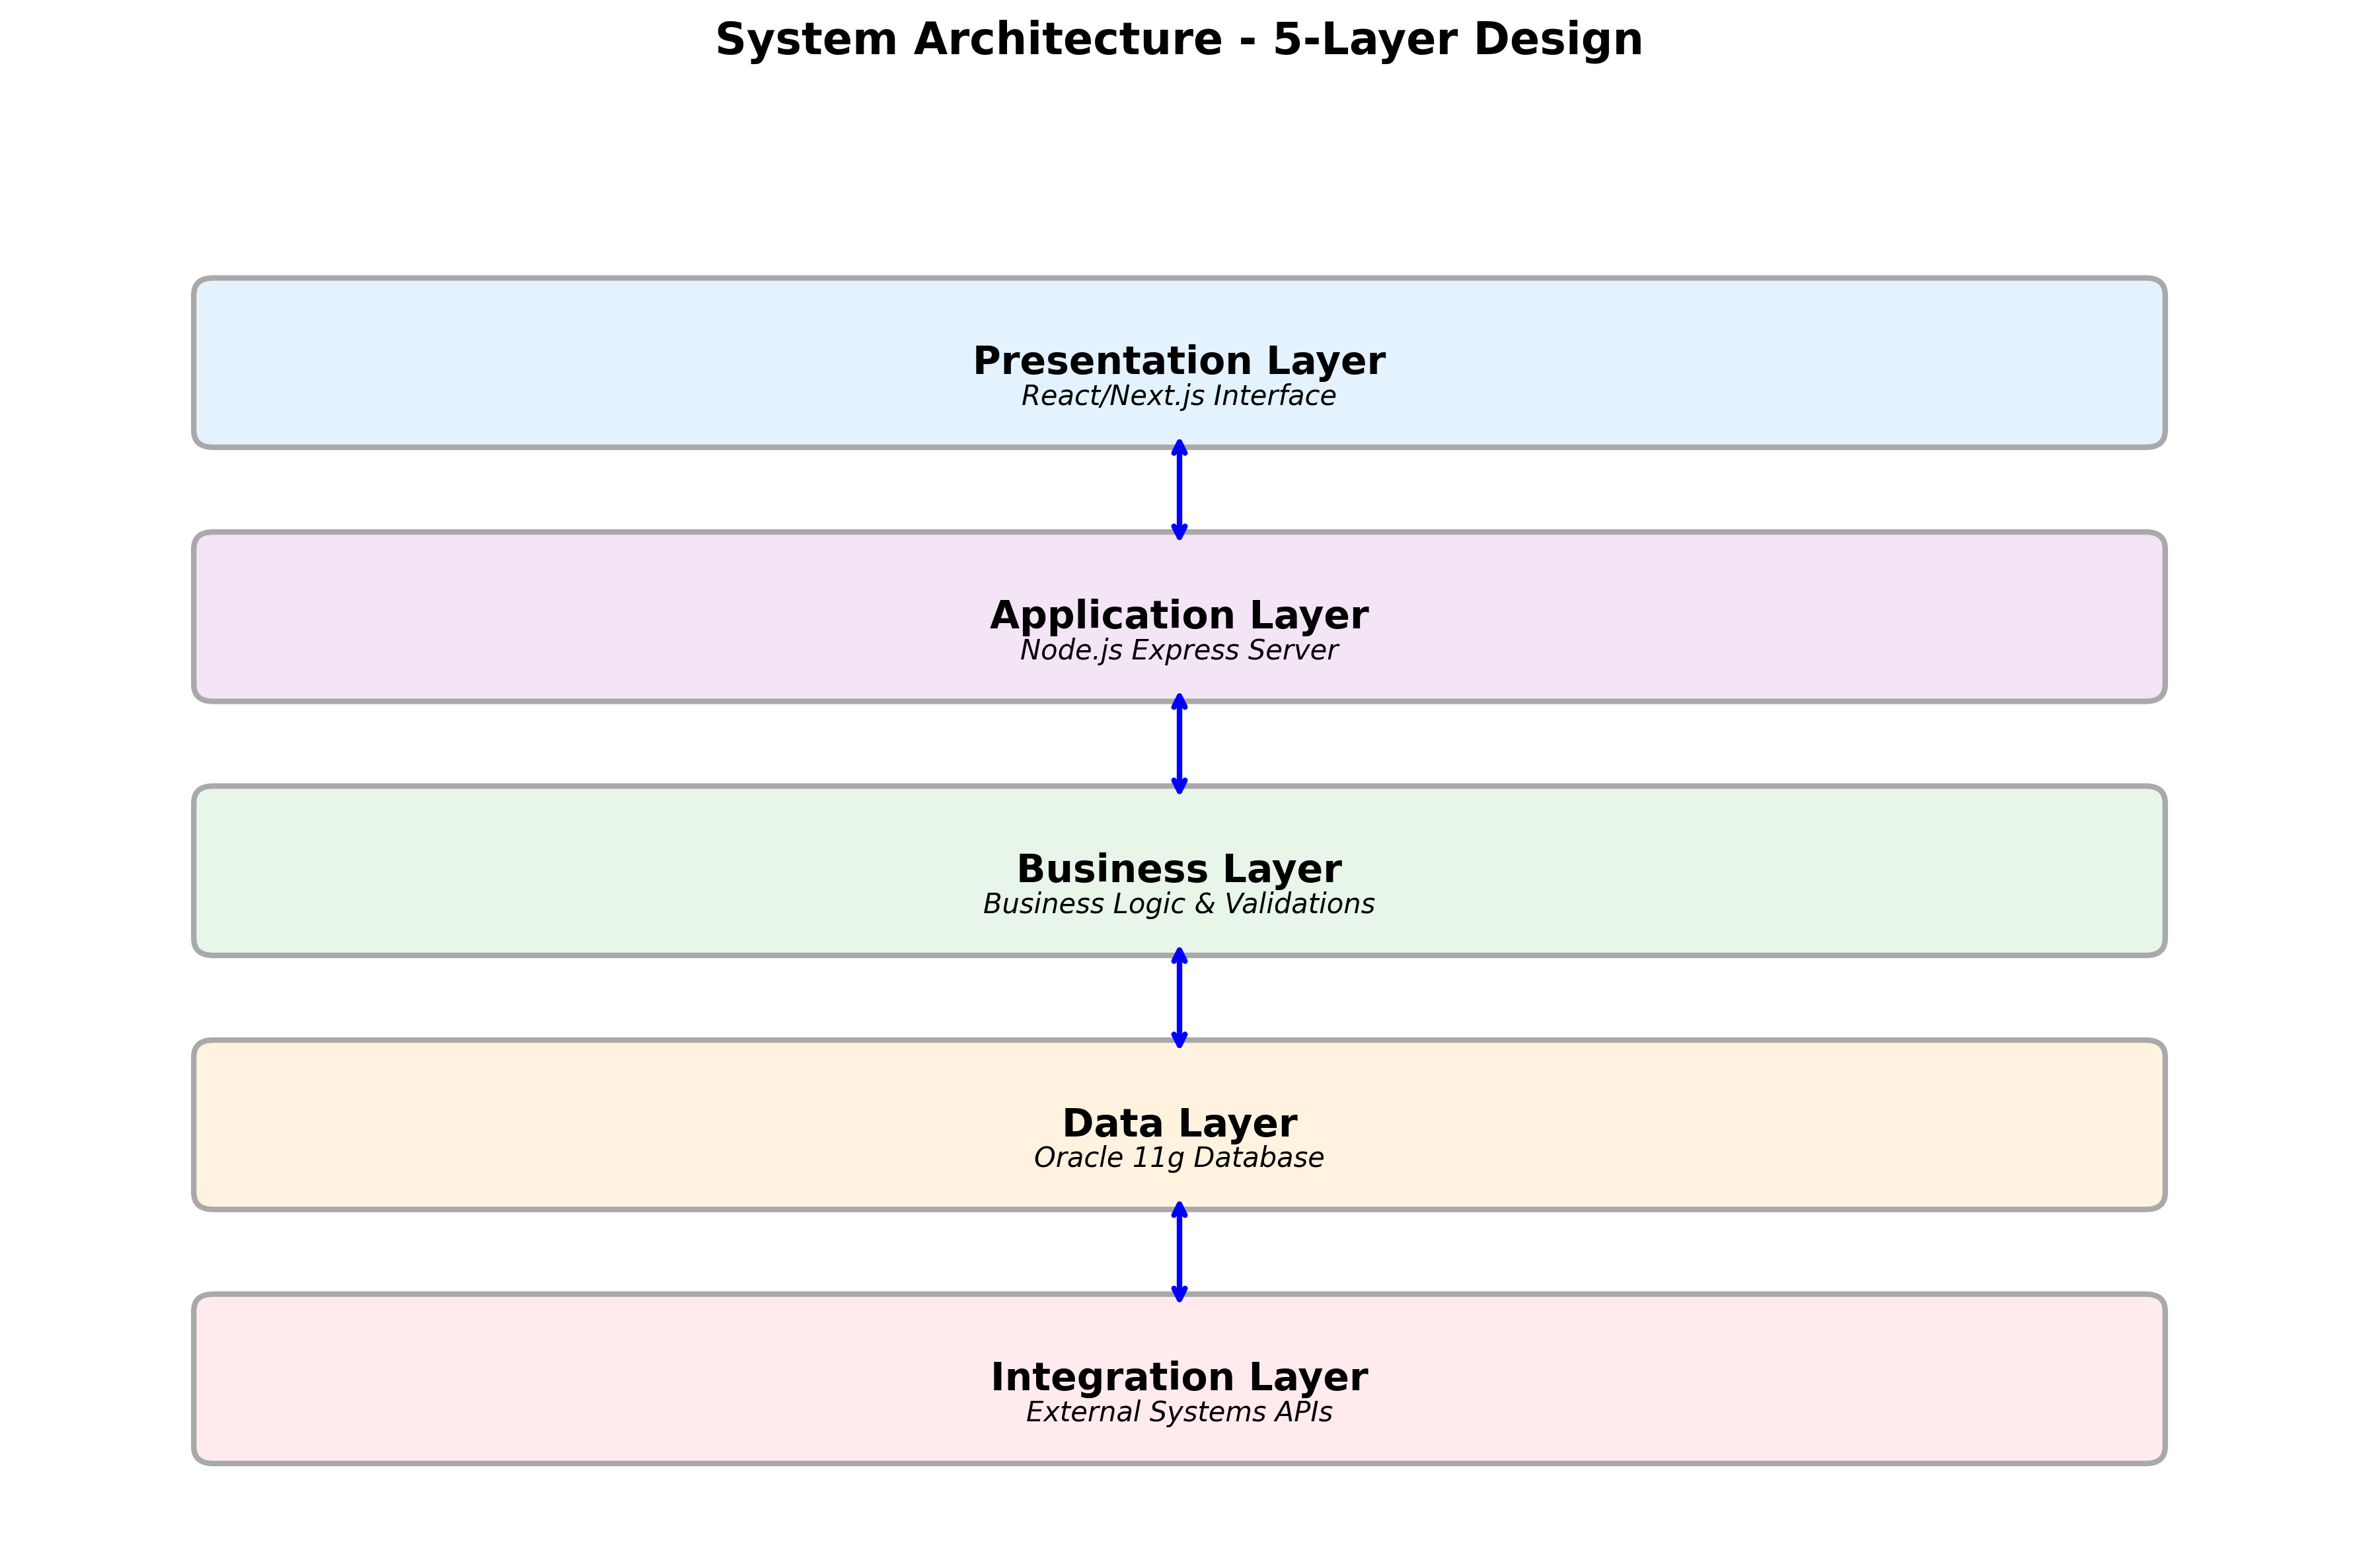
\includegraphics[width=0.95\textwidth]{images/generated/system_architecture.png}
    \caption{Layered architecture of the medication management system, detailing internal components and integrations with external systems.}
    \label{fig:architecture}
\end{figure}

The proposed architecture is organized into five distinct layers. The \textit{Presentation Layer}, built with React and Next.js, provides a responsive and intuitive \gls{ui}. It communicates with the \textit{Application Layer} (Node.js/Express), which orchestrates \glspl{api} requests. Core clinical intelligence resides in the \textit{Business Logic Layer}. Data persistence is handled by the \textit{Data Layer}, using an Oracle database, while the \textit{Integration Layer} provides secure RESTful interfaces for communication with other hospital systems.

Key components include robust authentication (e.g., LDAP-backed \gls{sso}) with granular role-based access control. The e-prescription module includes real-time clinical decision support (\gls{cdss}), aiming to reduce prescribing errors by validating prescriptions against a knowledge base for potential \gls{ddi} and allergies, a strategy supported in the literature \cite{bates2014}. The pharmaceutical validation system is designed to provide a complete and immutable audit trail, enhancing accountability.

\section{Performance and Quality Benchmarks}

Rigorous performance and quality assurance are central to the development methodology. Targeted optimizations aim for low-latency interactions and responsive user experience in clinical settings (e.g., sub-second feedback for critical interactions), using techniques such as efficient querying, caching and judicious precomputation \cite{nielsen2012}.

A primary technical objective is to achieve seamless integration with existing hospital systems, with robust validation and transformation pipelines to minimize synchronization errors. Furthermore, a disciplined testing and refactoring effort increases automated test coverage for critical paths, and the frontend aligns with \gls{wcag} 2.1 Level AA.

\paragraph{Process Standardization and Bedside Administration Alignment}
Expected results include progress toward standardized digital pathways across the medication cycle (protocolized steps, mandatory data elements, and embedded decision checks) and alignment with bedside administration practices (eMAR/BCMA; Section~\ref{sec:emar_bcma}). These outcomes are evidenced through updated flows, UI affordances, and traceability/audit capabilities rather than fixed numerical targets.

\section{Evaluation Plan and Expected Clinical Impact}

Evaluation is planned through a pilot phase at \gls{scmvv} to assess real-world impact. Adoption levels and platform reliability are tracked as key indicators; high availability appropriate for clinical use is a design objective and is confirmed during evaluation \cite{nkenyereye2016}. Comparisons reference the baseline synthesized from legacy analyses (Chapter~\ref{chap:Results}, Section "Baseline from Legacy Analyses").

The intended outcome centers on patient safety. As illustrated conceptually in Figure~\ref{fig:error-reduction}, the project targets a substantial reduction in prescribing and validation errors, consistent with effects reported in the literature \cite{radley2013, bates2014}. End-to-end traceability is expected to shorten incident investigations; concrete magnitudes are established from collected evidence during evaluation.

\begin{figure}[htbp]
    \centering
    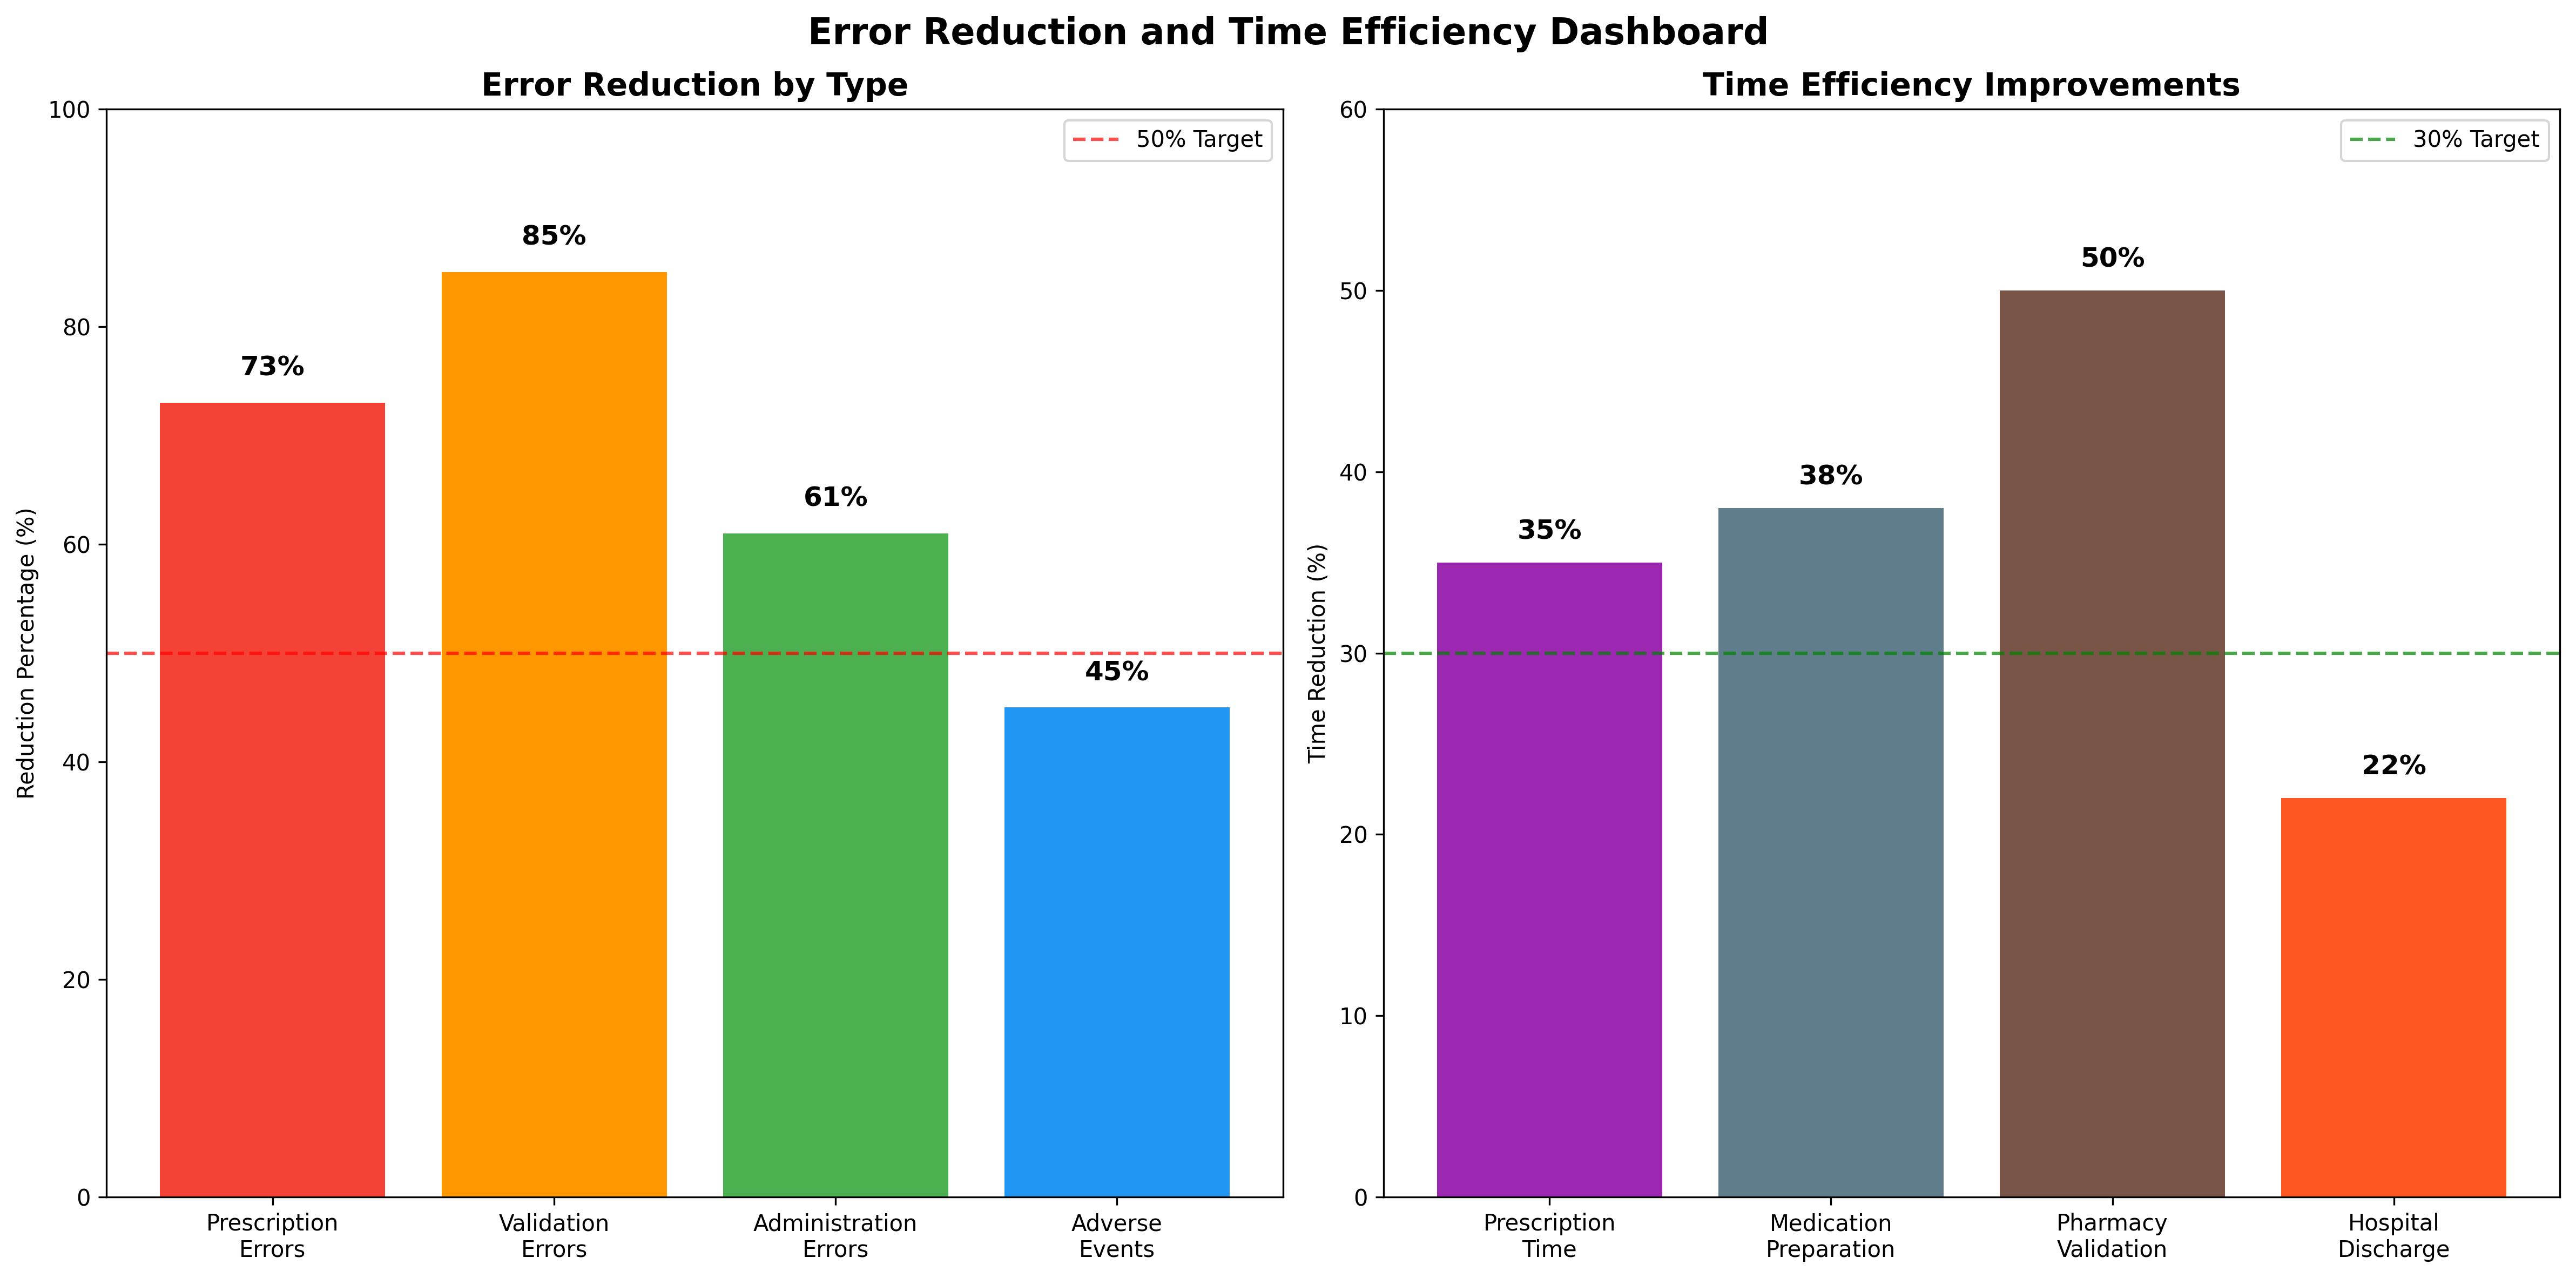
\includegraphics[width=0.95\textwidth]{images/generated/error_reduction_dashboard.png}
    \caption{Dashboard illustrating the reduction in medication errors and improvements in process efficiency following system implementation.}
    \label{fig:error-reduction}
\end{figure}

Operational efficiency gains are also expected. The system streamlines clinical workflows to reduce time to prescribe and validate and to decrease clarification requests, thereby freeing clinical time for patient care \cite{austin2018}. Specific magnitudes are treated as targets to be validated empirically. Alignment with bedside administration practices (eMAR/BCMA; Section~\ref{sec:emar_bcma}) and standardized digital pathways (Section~\ref{sec:process_standardization}) is pursued as part of the objectives.

\section{User Acceptance Evaluation}

High user acceptance is critical for success. User acceptance is evaluated with the System Usability Scale (SUS) and complementary qualitative methods. An acceptable goal is a "Good" or better SUS outcome for the target user groups, to be confirmed by the study \cite{lewis2018}.

Qualitative feedback is collected through semi-structured interviews and focus groups with physicians, pharmacists, and nurses (Figure~\ref{fig:user-satisfaction}). This feedback is analyzed to assess confidence in the system, perceived safety improvements, and workflow clarity. Training time for new users is also monitored with the objective of meaningful reduction compared to the legacy system.

\begin{figure}[htbp]
    \centering
    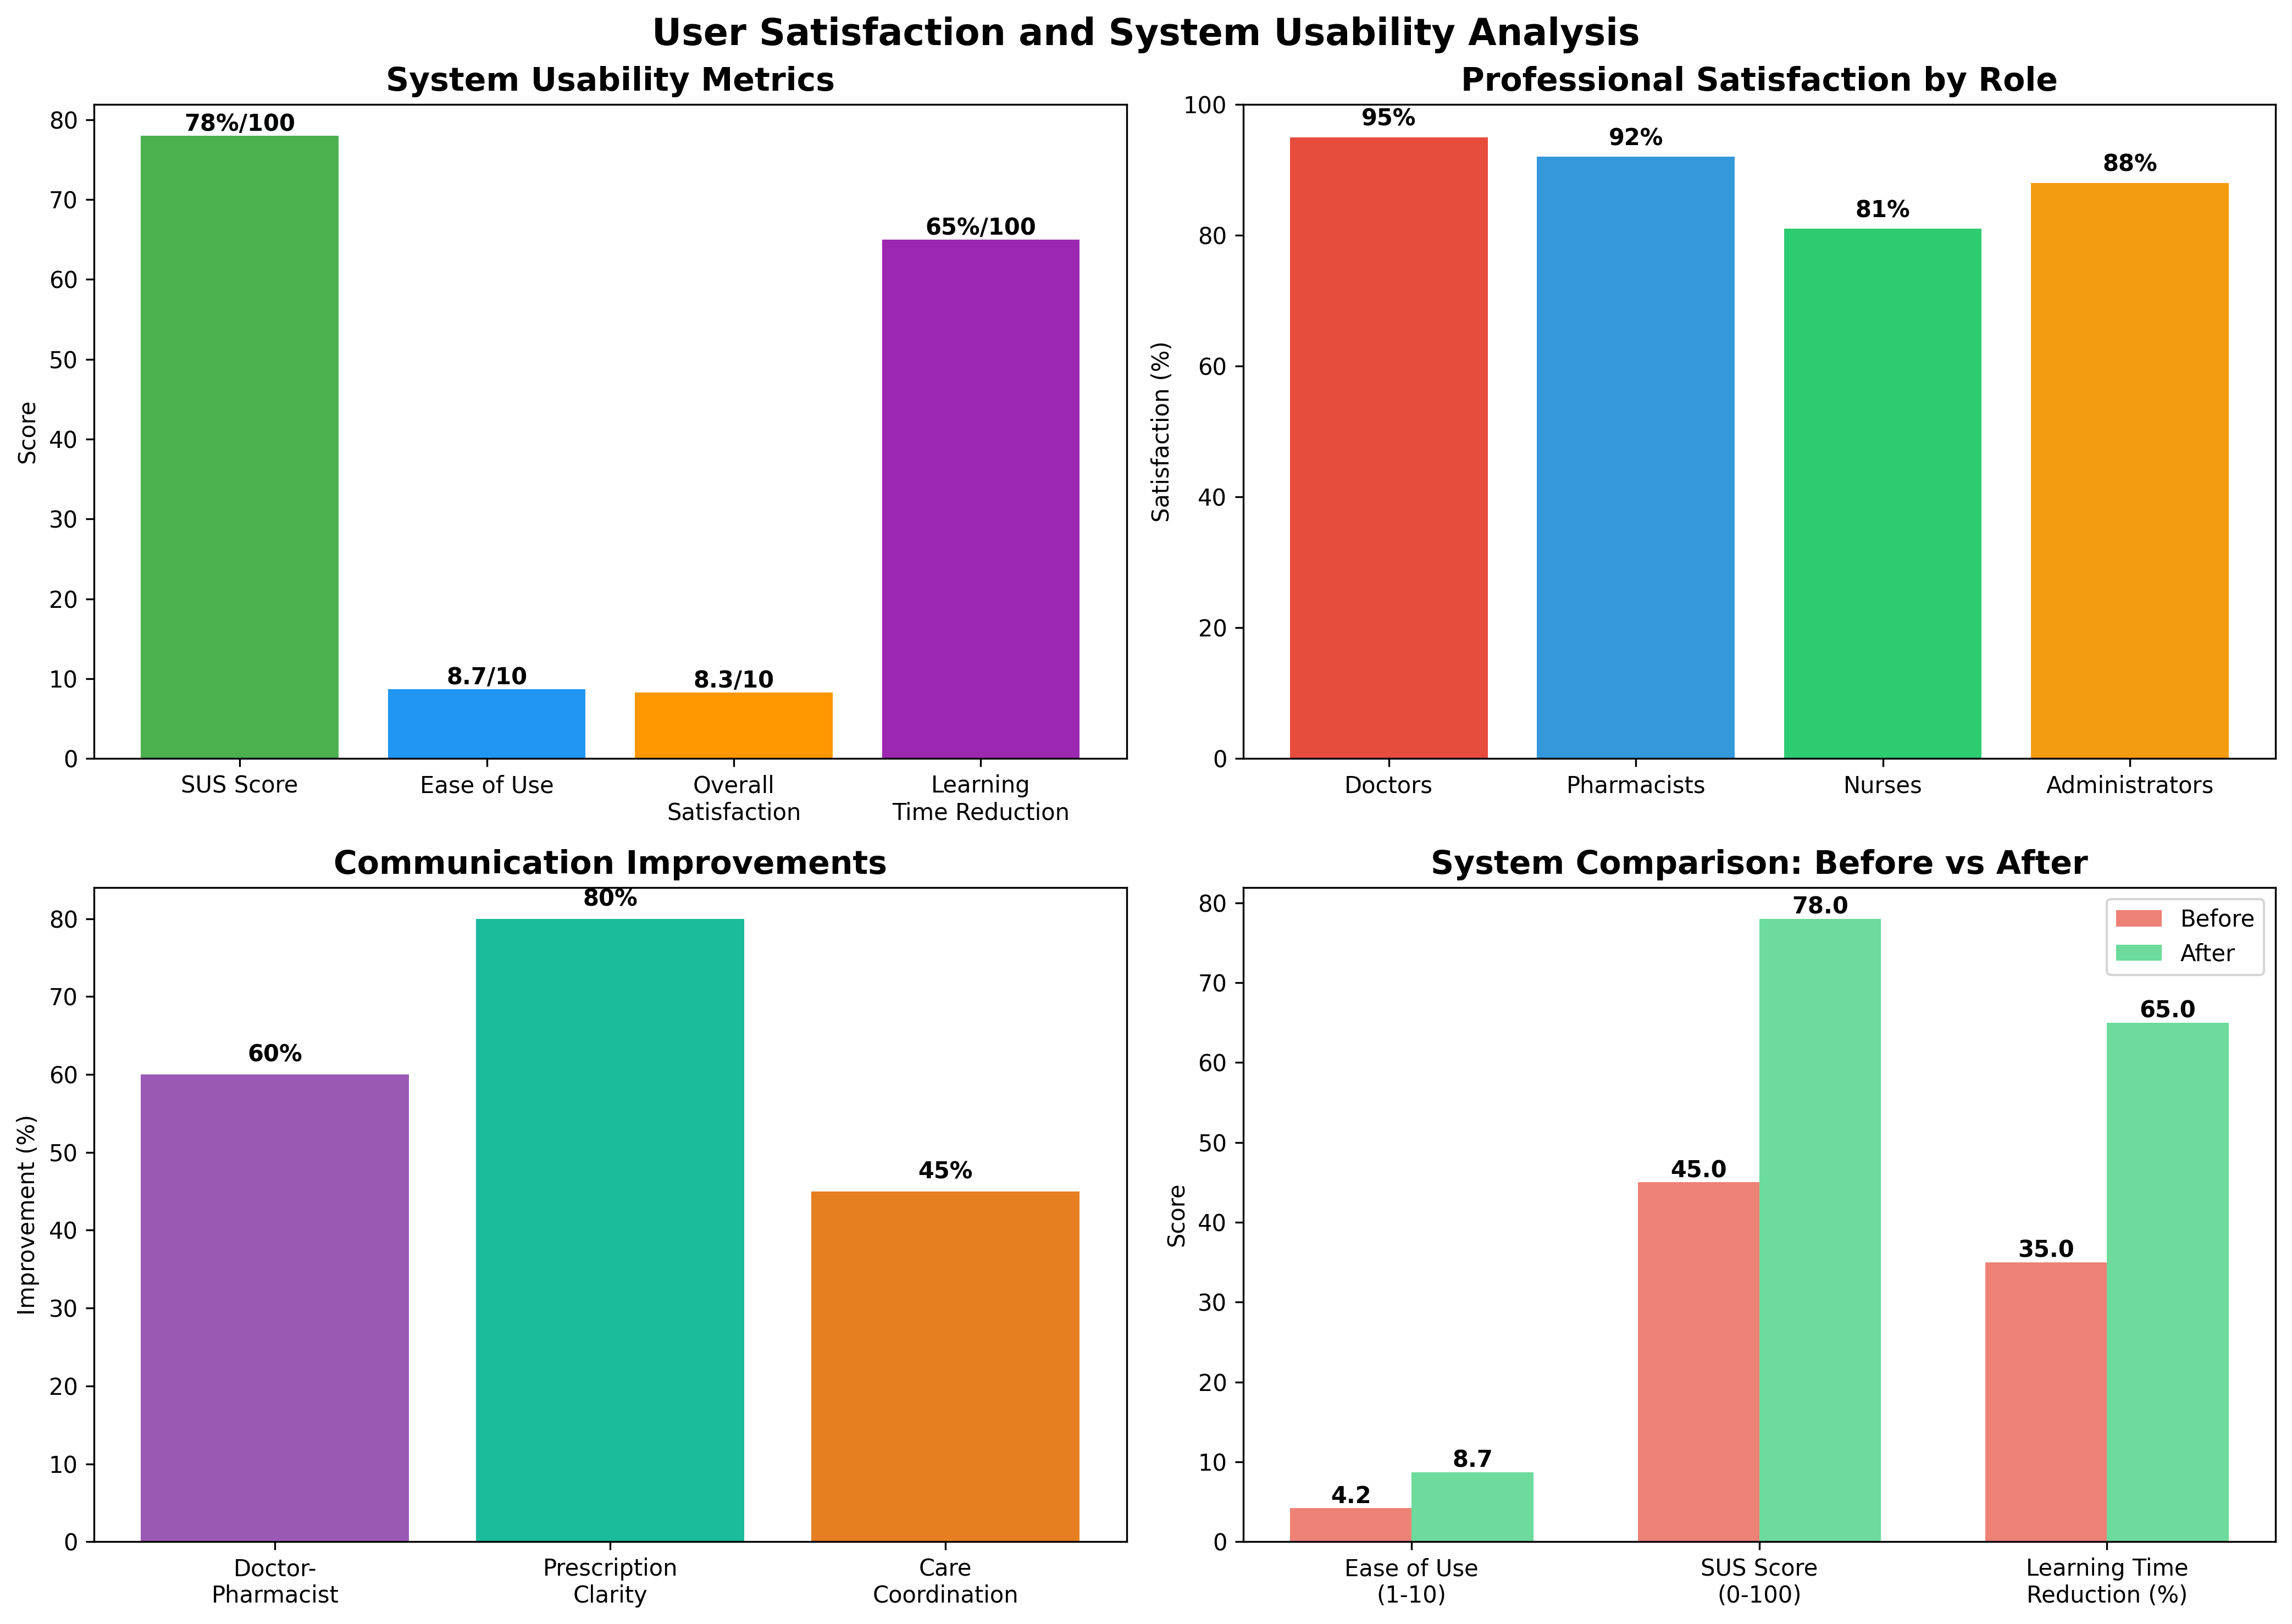
\includegraphics[width=0.95\textwidth]{images/generated/user_satisfaction.png}
    \caption{Comprehensive analysis of user satisfaction, including usability metrics, satisfaction ratings by professional category, and communication improvements.}
    \label{fig:user-satisfaction}
\end{figure}

\section{Expected Financial Impact and Future Viability}

A cost-benefit analysis is conducted as part of the evaluation to determine financial impact. Based on efficiency gains and reduced costs associated with medication errors, Figure~\ref{fig:roi-analysis} summarizes an indicative ROI model; the specific payback period is estimated and validated with study data \cite{adler2021}. Coupled with planned scalability and the strategic roadmap (Figure~\ref{fig:future-roadmap}), this supports long-term viability and potential expansion.

\begin{figure}[htbp]
    \centering
    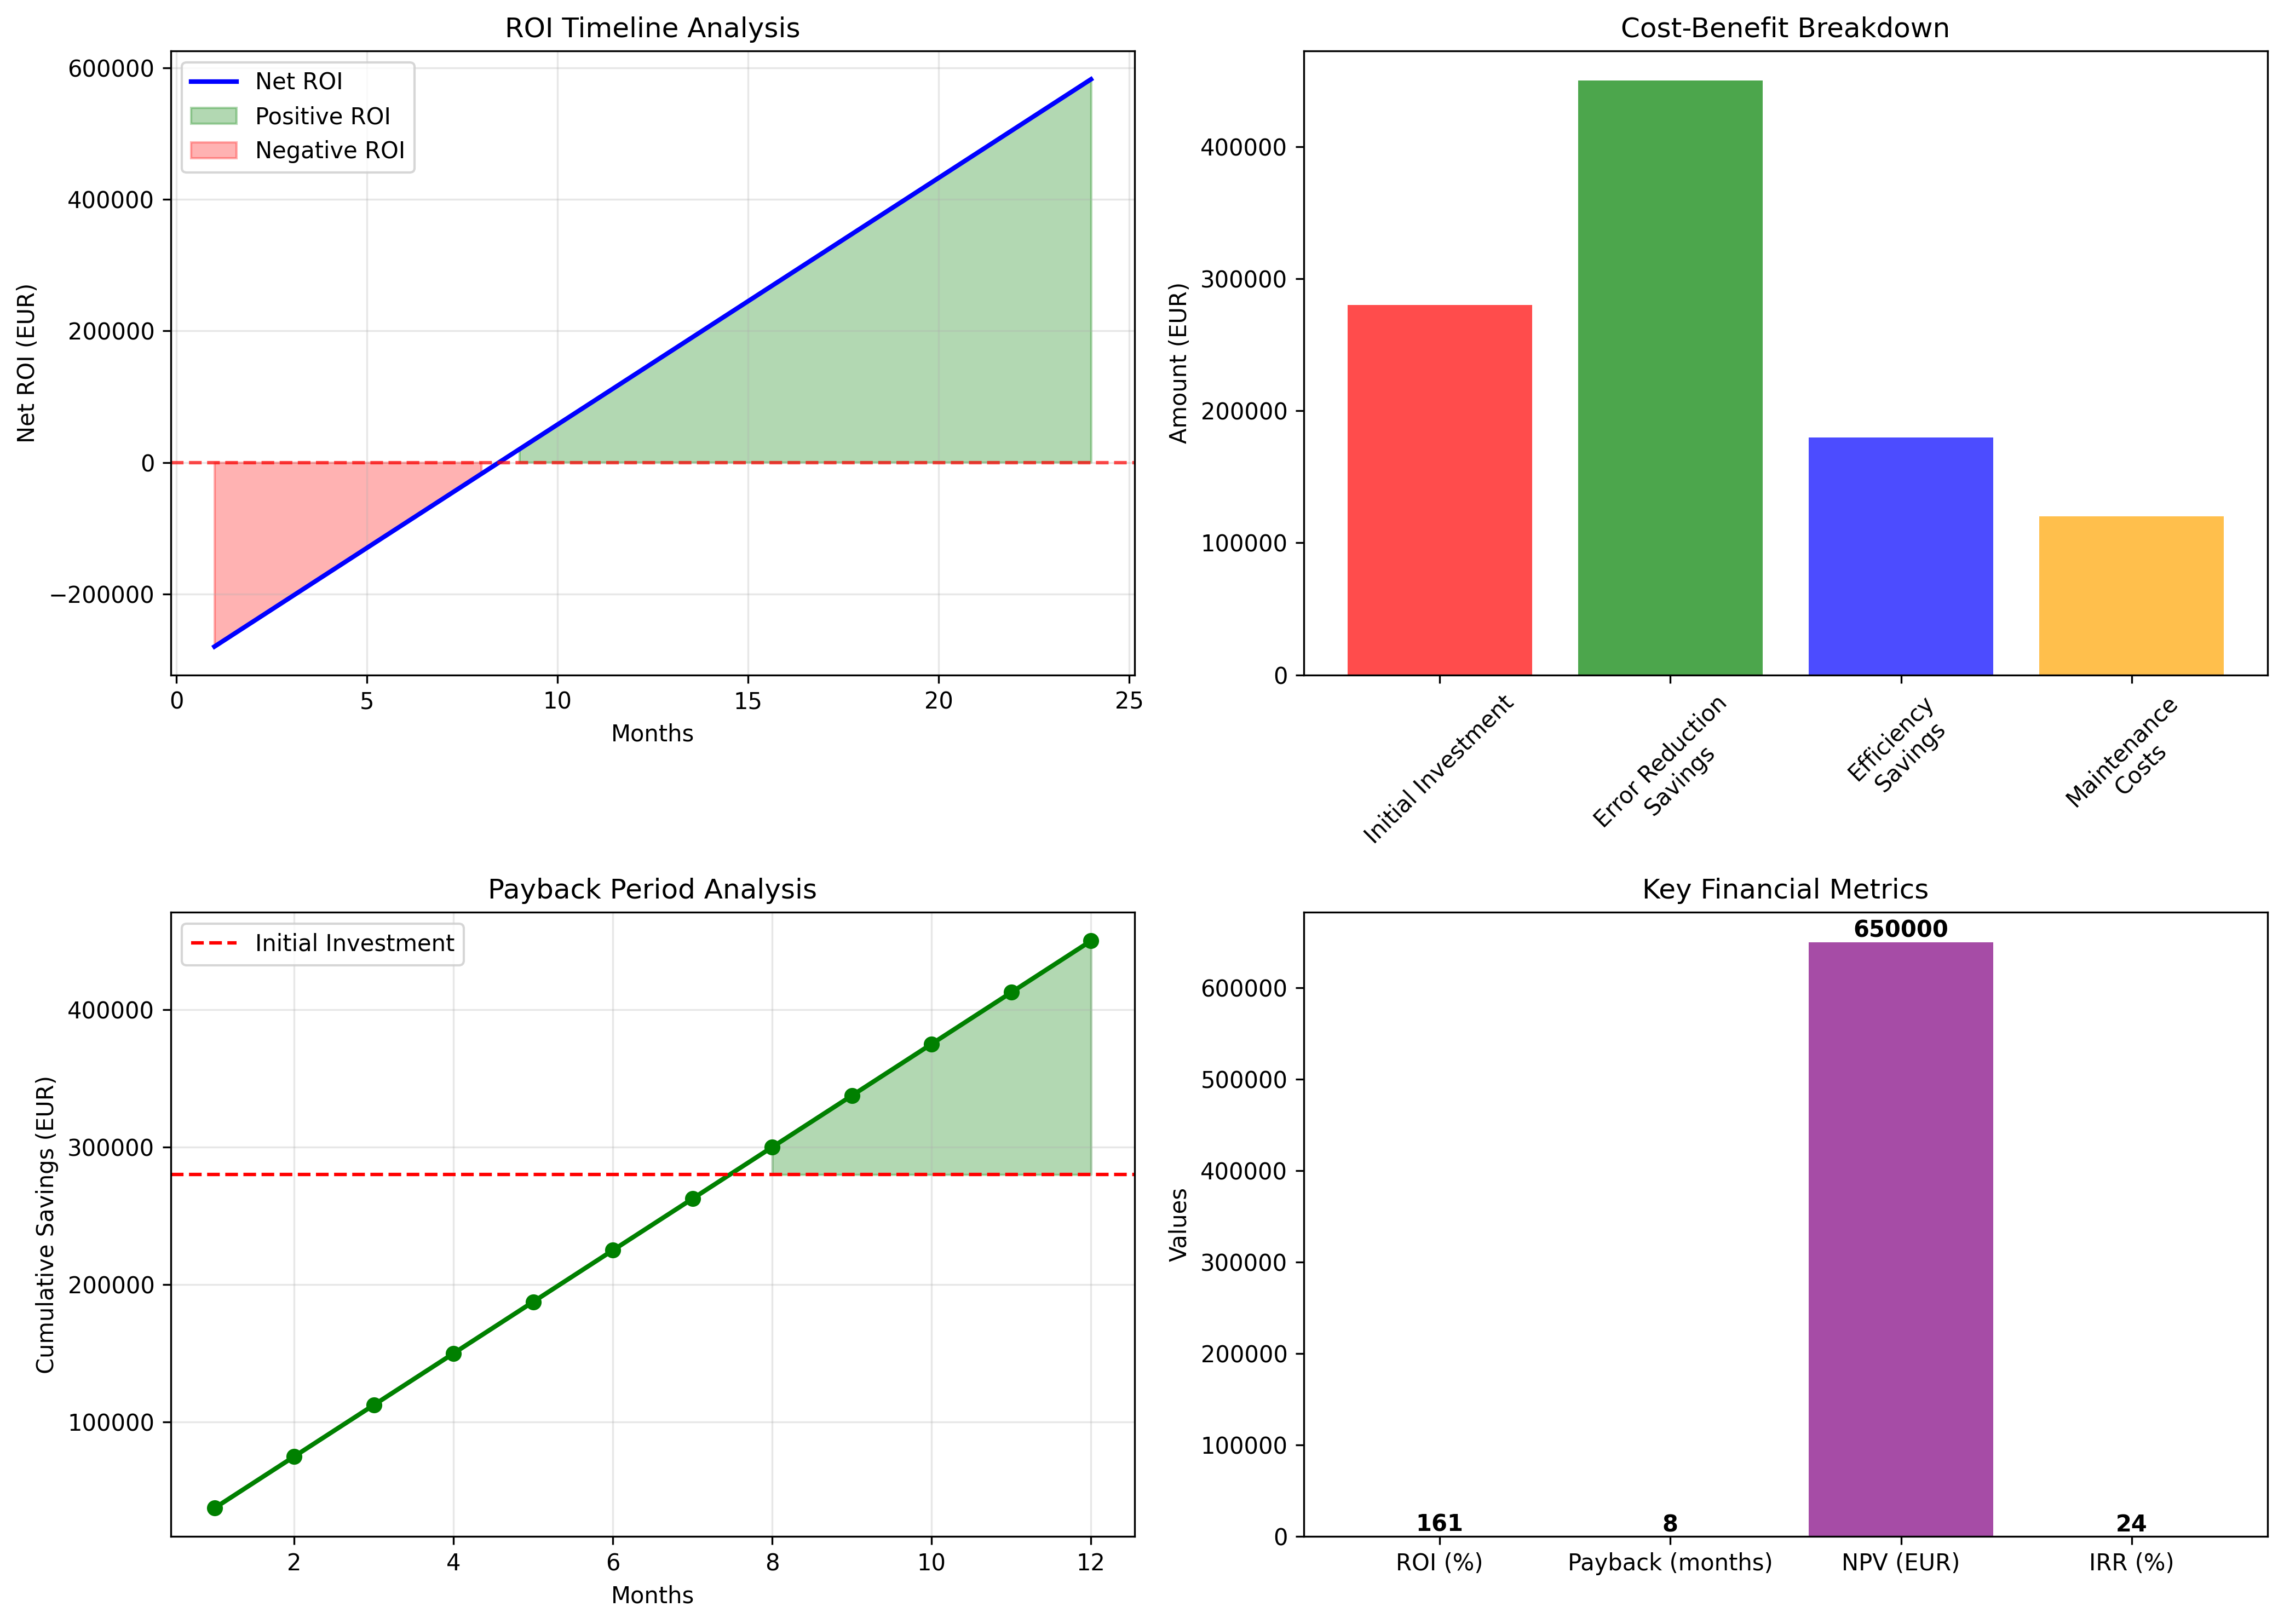
\includegraphics[width=0.95\textwidth]{images/generated/roi_analysis.png}
    \caption{Cost-benefit analysis, including investment breakdown, ROI timeline, and payback period calculation.}
    \label{fig:roi-analysis}
\end{figure}

\begin{figure}[htbp]
    \centering
    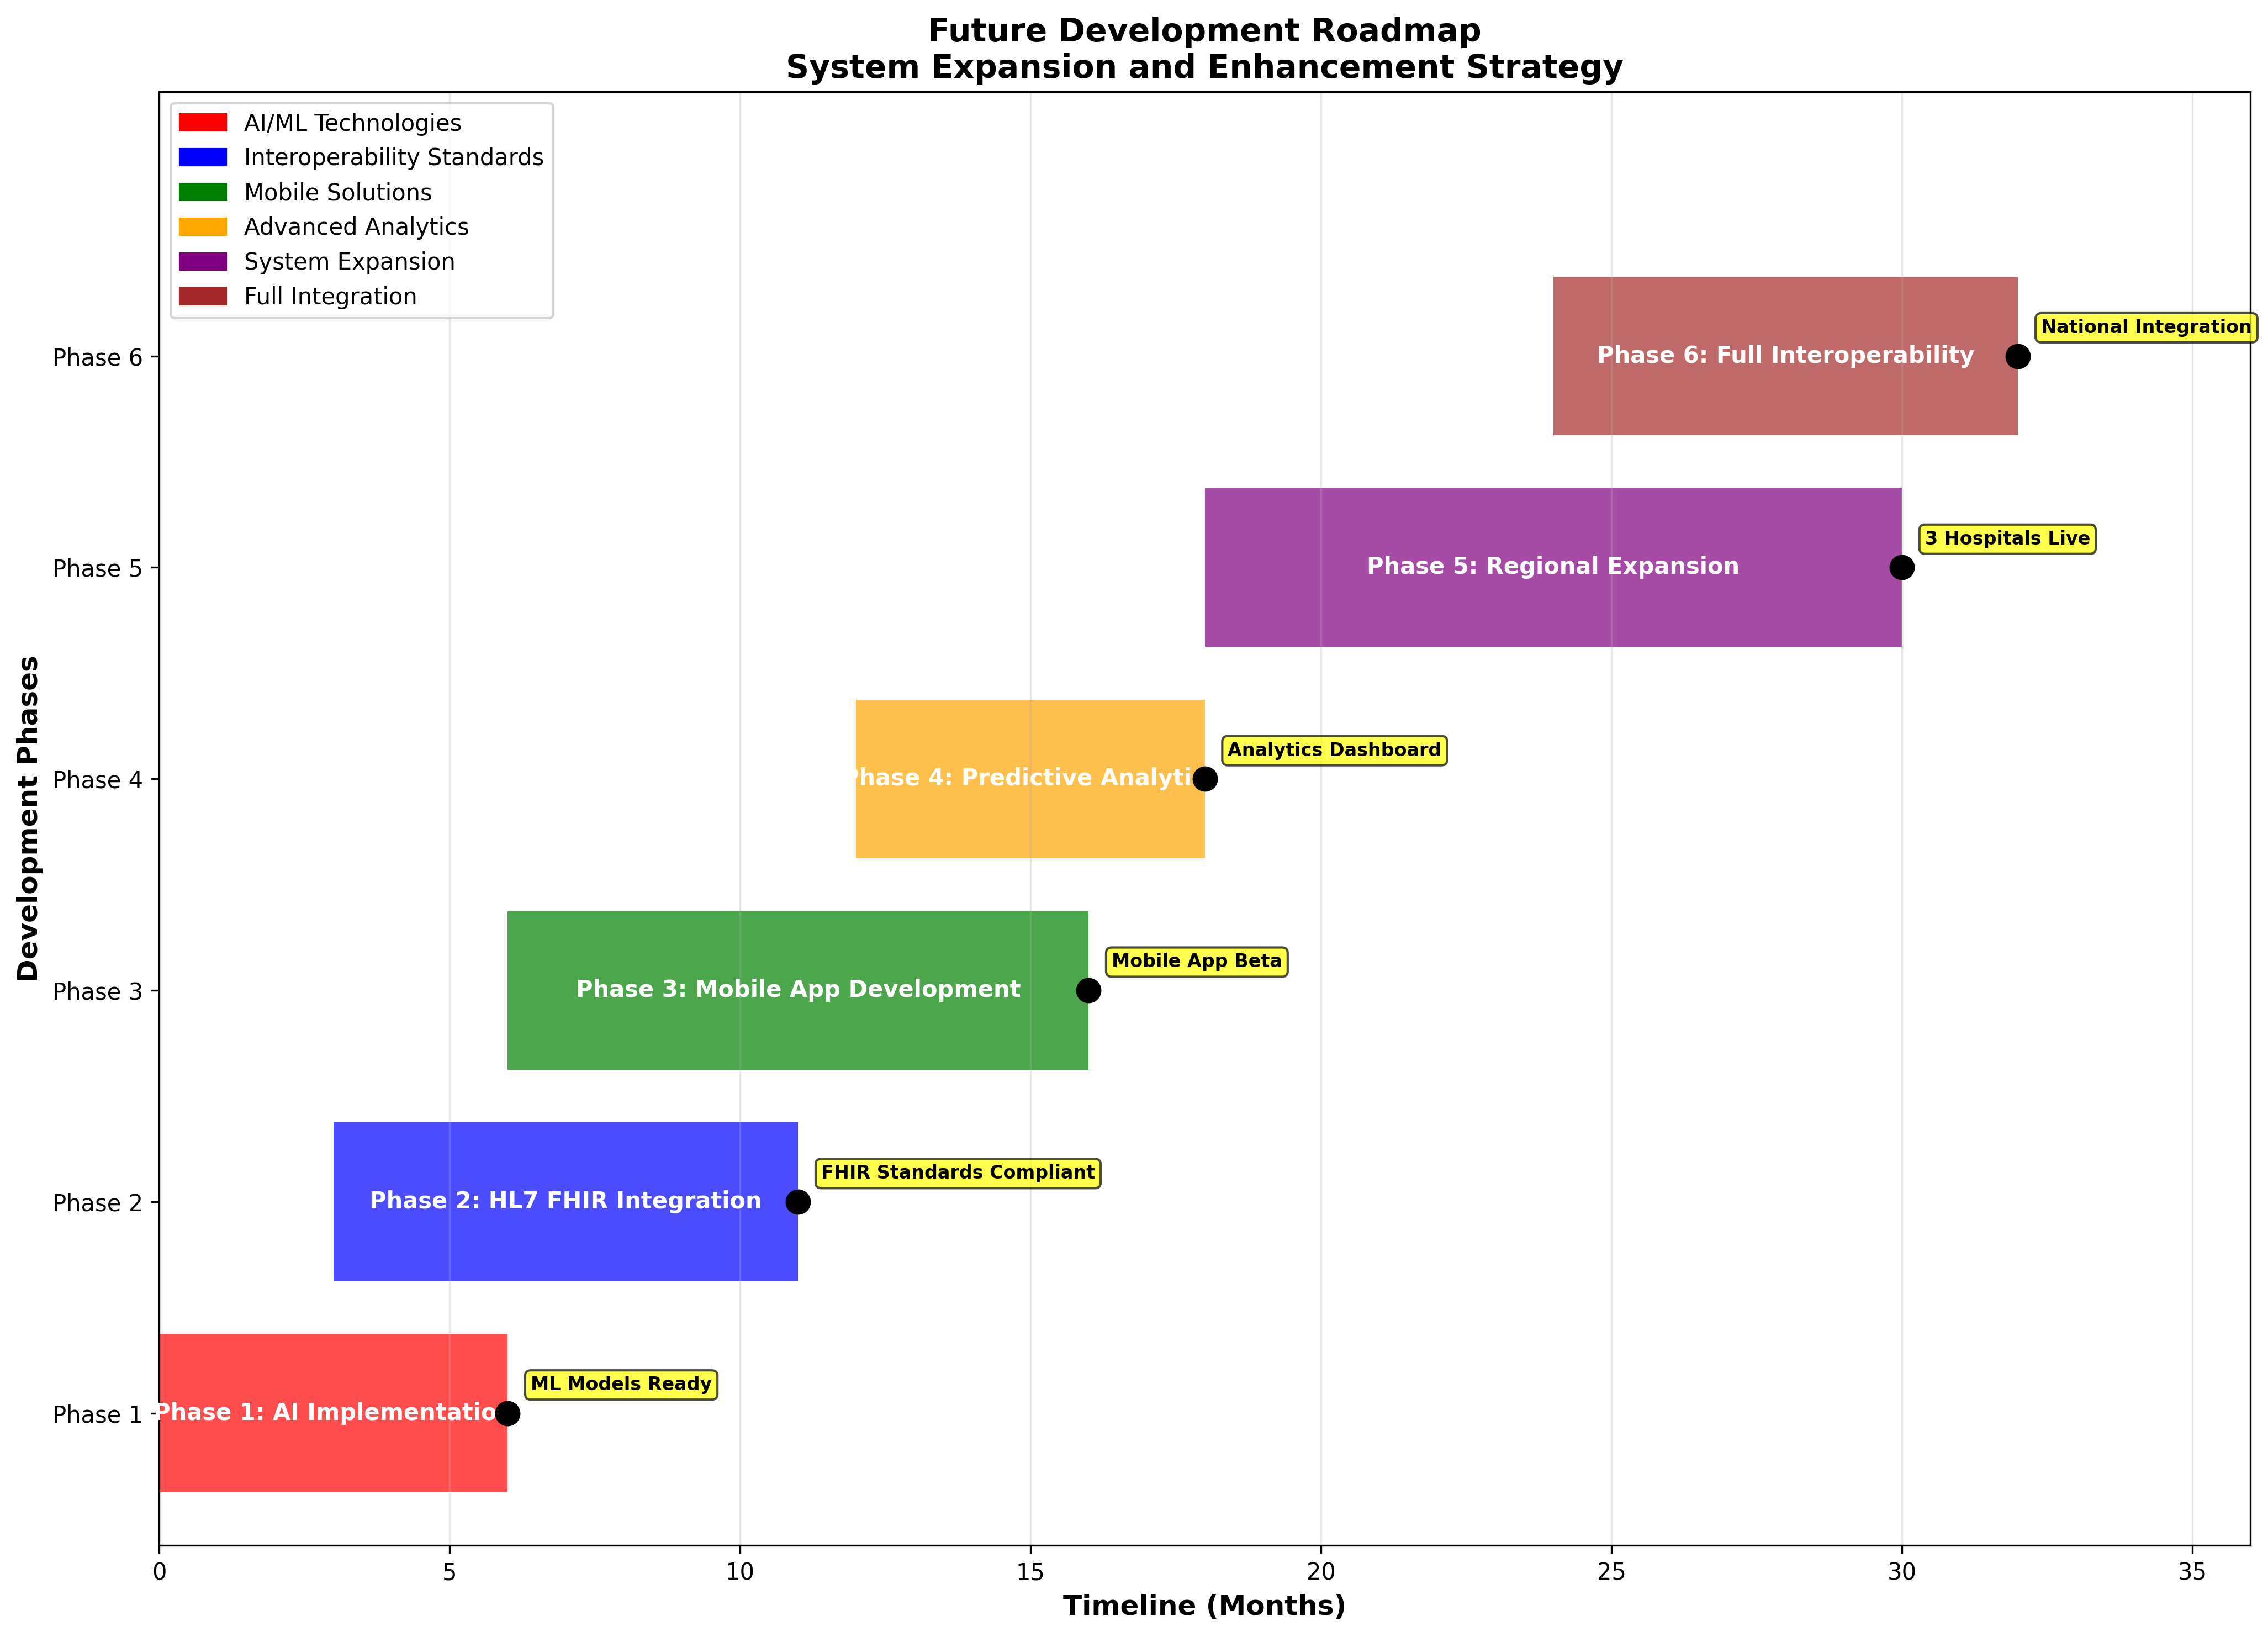
\includegraphics[width=0.95\textwidth]{images/generated/future_roadmap.png}
    \caption{18-month future development roadmap, including AI/ML features, FHIR integration, mobile application development, and regional expansion.}
    \label{fig:future-roadmap}
\end{figure}

\subsection{Key Performance Indicators and Evaluation Scenarios}
\label{sec:KPIs}

To anchor the evaluation in the operational realities of \gls{scmvv}, the pilot focuses on a set of Key Performance Indicators (KPIs), grounded in challenges described by clinical staff and contextualized by fragmentation issues in the Portuguese NHS \cite{goiana2024portuguese, nunes2021articulacao}.

\subsubsection{Patient Safety and Clinical Quality}
The evaluation primarily focuses on reduction in medication errors. This is measured by comparing pre- and post-intervention error rates (e.g., incorrect dosage, wrong medication, missed administrations), using appropriate sample sizes and definitions agreed with stakeholders. Adherence to protocols is assessed by auditing system logs to quantify compliance with integrated clinical decision support rules.

\subsubsection{Operational Efficiency}
To measure gains in efficiency, the study analyzes time-in-motion for clinical staff, observing the end-to-end process of medication administration before and after system introduction. Additionally, pharmaceutical validation time is measured from prescription entry to final validation, comparing performance against the current multi-system workflow.

\subsubsection{System Integration and Data Integrity}
The success of integration is quantified by measuring reduction in data redundancy and discrepancies. This is achieved through comparative analysis of patient records across relevant systems before and after implementation, identifying inconsistencies in key data fields (e.g., patient identifiers, active medication lists) to demonstrate improvement in data coherence, a known challenge in fragmented health information environments \cite{pinto2016identification}. 